\documentclass[class=book, crop=false, oneside]{standalone}
\usepackage[subpreambles=true]{standalone}

\usepackage{../../style}

\graphicspath{{./images/}}

% arara: pdflatex: { synctex: yes, shell: yes }
% arara: latexmk: { clean: partial }
%! arara: clean: { extensions: [sta] }
\begin{document}
\chapter*{Introduzione}
% \addcontentsline{toc}{chapter}{Introduzione} \markboth{INTRODUZIONE}{}

Quella che il lettore sta approcciando è una dispensa che raccoglie, riorganizza e riespone l'intero contenuto del corso di \emph{calcolatori} tenuto nell'Università degli studi di Trento durante il secondo semestre dell'anno accademico 2018/2019. La repository del progetto può essere raggiunta tramite il seguente link: \url{https://github.com/Samaretas/Appunti-Calcolatori}.

Le risorse utilizzate sono state le slides fornite dal professor Giovanni Iacca (corso dispari) durante le lezioni e integrate dalle sue spiegazioni, la dispensa "Piccola introduzione al linguaggio Assembly e simili amenità" del professor Luca Abeni, le lezioni dell'esercitatore Fabiano Zenatti e svariate risorse online per dirimere alcune lievi questioni non meritevoli del disturbo ai professori. L'elaborato è stato suddiviso in capitoli che seguono il partizionamento proposto dal professore e, successivamente, in sezioni e sottosezioni per questioni di agilità consultativa. I singoli argomenti vengono presentati nell'ordine e modalità proposti dal professore (all'infuori di sporadici casi in cui gli autori hanno proposto una maniera da loro ritenuta più fruibile per il target di riferimento), corredati da immagini e codici commentati dove possibile.

Nel momento della stesura questa dispensa si propone di essere autoconsistente nell'ottica della preparazione dell'esame di fine corso, ossia lo studente potrebbe potenzialmente usare questo testo come unica risorsa ed essere ampiamente in grado di superare con successo l'esame. Quest'ultimo, alla data attuale, consiste in 12 domande a risposta multipla, ciascuna delle quali del valore di \(2.75\) punti, per un totale di \(33\). Si tenga presente che ogni risposta errata comporta una decurtazione di \(0.55\) punti dal totale; risposte considerate nulle non comporteranno alcuna penalità.

\emph{Nota bene}: a seguito di alcune modifiche apportate al programma del corso per l'anno accademico \(2019\)-\(2020\), questo elaborato non può più dirsi autoconsistente. Gli autori invitano pertanto i futuri studenti del corso che volessero contribuire ad aggiornare la dispensa a contattarli per ricevere istruzioni su come partecipare al progetto.

Ecco una breve presentazione degli autori; per raggiungere il profilo GitHub di ciascuno è sufficiente cliccare sul relativo nome; ognuno dei tre, a turno, ha curato l'esposizione dei singoli capitoli.
\vskip 10pt
\begin{minipage}{.6\textwidth}
    \begin{itemize}
		\item \emph{\href{https://github.com/FrancescoBozzo}{Francesco Bozzo}}: leader e responsabile del progetto, ha frequentato il liceo scientifico indirizzo scienze applicate G.B. Quadri di Vicenza e successivamente si è iscritto all'Università di Trento, corso di laurea in informatica. Nel progetto si è dedicato principalmente alla parte più tecnica, risolvendo ogni volta qualsiasi problema \LaTeX\ potesse presentare, il che gli ha giustamente procurato il titolo di campione della Lega Pokémon della regione di Trentoh.
	\end{itemize}
\end{minipage}
\hspace{.1\textwidth}
\begin{minipage}{.4\textwidth}
	{%
		\setlength{\fboxsep}{0pt}%
		\setlength{\fboxrule}{1pt}%
		\fbox{
\includegraphics[scale=0.30]{Fra.jpg}}%
	}%
\end{minipage}
\vskip 20pt
\begin{minipage}{.3\textwidth}
	{%
		\setlength{\fboxsep}{0pt}%
		\setlength{\fboxrule}{1pt}%
		\fbox{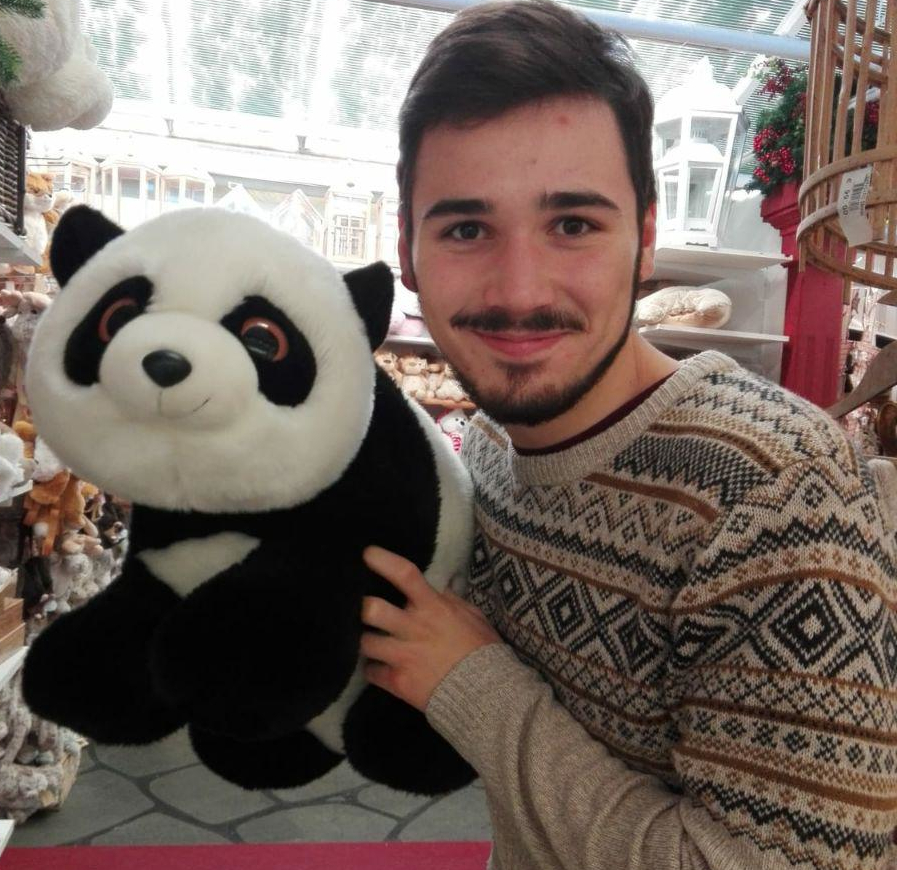
\includegraphics[scale=0.19]{Sam.jpg}}%
	}%
\end{minipage}
\hspace{.01\textwidth}
\begin{minipage}{.7\textwidth}
    \begin{itemize}
		\item \emph{\href{https://github.com/Samaretas}{Samuele Conti}}: ha frequentato scienze applicate a Verona, quindi non un liceo vero, e da un anno a questa parte frequenta l'Università di Trento dove ha raggiunto la notorietà per mezzo delle sue memorabili sbronze. Particolarmente notevoli i suoi errori di ortografia e la sua incapacità di formulare pensieri in modo ordinato. Tutto sommato però è un bravo ragazzo, ve lo raccomando.
	\end{itemize}
\end{minipage}
\vskip 20pt
\begin{minipage}{.6\textwidth}
    \begin{itemize}
		\item \emph{\href{https://github.com/filippodaniotti}{Filippo Daniotti}}: dopo aver frequentato il liceo classico Antonio Scarpa, si è iscritto al corso di laurea in informatica presso l'Università di Trento, già da questa premessa si deduce quindi il suo forte carattere masochista. Ha curato la revisione ortografica e morfosintattica del progetto, il commento dei codici e la stesura di quest'introduzione. Inoltre ha sempre dimostrato una grande passione per l'utilizzo del tool \LaTeX\ (qui ritorna il carattere masochista) e molti ritengono che per questa ragione sia il classico tipo che alle feste rimane solo in un angolino a compiangere se stesso.
	\end{itemize}
\end{minipage}
\hspace{.1\textwidth}
\begin{minipage}{.4\textwidth}
	{%
		\setlength{\fboxsep}{0pt}%
		\setlength{\fboxrule}{1pt}%
		\fbox{
\includegraphics[scale=.50]{Pips.jpg}}%
	}%
\end{minipage}

\end{document}
